\section{Singularities}

\begin{frame}[standout, plain, noframenumbering]
    Singularities

    % \medskip

    % \footnotesize
    % Sam Greydanus \quad Misko Dzamba \quad Jason Yosinski
\end{frame}

\begingroup
\small


\begin{frame}
    \frametitle{Singularities}

    \begin{itemize}
        \item The $6 \times n$ Jacobian $J(q)$ defines a mapping \[ \xi =
        J(q)\dot{q} \] between the vector $\dot{q}$ of joint velocities and the
        vector $\xi = (v, \omega)$ of end effector velocities. In other words,
        \[ \xi = J_1 \dot{q}_1 + J_2 \dot{q}_2 + \cdots + J_n \dot{q}_n. \]
        \item Since $\xi \in \mathbb{R}^6$, it is necessary that $J$ have six 
        linearly independent columns for the end effector to be able to achieve 
        any arbitrary velocity.
        \item Thus, when $\rank J = 6$, the end effector can execute any
        arbitrary velocity. Notice that for a matrix $J \in \mathbb{R}^{6 \times
        n}$, it is always the case that $\rank J \leq \min{(6, n)}$.
    \end{itemize}
\end{frame}


\begin{frame}
    \frametitle{Singularities}

    \begin{itemize}
        \item The rank of the manipulator Jacobian will depend on the
        configuration $q$.
        \item Configurations for which $\rank J(q)$ is less than its maximum
        value are called \textbf{singularities} or \textbf{singular
        configurations}.
        \item Identifying manipulator singularities is important because \ldots
        \begin{itemize}
            \footnotesize{
            \item Singularities represent configurations from which certain
            directions of motion may be unattainable.
            \item At singularities, bounded end effector velocities may
            correspond to unbounded joint velocities.
            \item At singularities, bounded joint torques may correspond to
            unbounded end effector forces and torques.
            \item Singularities often correspond to poitns on the boundary of
            the manipulator workspace, that is, to points of maximum reach of
            the manipulator.
            \item Singularities correspond to points in the manipulator
            workspace that may be unreachable under small perturbations of the
            link parameters, such as length, offset, etc.
            }
        \end{itemize}
    \end{itemize}
\end{frame}


\begin{frame}
    \frametitle{Decoupling of Singularities}

    \begin{itemize}
        \item For manipulators with spherical wrists, determination of singular
        configurations may be decoupled into two simpler problems.
        \item The first problem is to determine so-called \textbf{arm
        singularities}, that is, singularities resulting from the motion of the
        arm, which consists of the first three or more links.
        \item The second problem is to determine the \textbf{wrist
        singularities} resulting from motion of the spherical wrist.
    \end{itemize}
\end{frame}


\begin{frame}
    \frametitle{Decoupling of Singularities}

    \begin{itemize}
        \item Consider the case that $n=6$, that is, the manipulator consists of 
        a $3$-DOF arm with a $3$-DOF spherical wrist.
        \item The Jacobian is a $6 \times 6$ matrix and a configuration $q$ is
        singular iff $\det J(q) = 0$.
        \item If we partition the Jacobian into $3 \times 3$ blocks as 
        \[ J = \begin{bNiceArray}{c|c}
            J_P & J_O
        \end{bNiceArray} = 
        \begin{bNiceArray}{c|c}[margin]
            J_{11} & J_{12} \\ \hline
            J_{21} & J_{22}
        \end{bNiceArray} 
        \]
        then, since the final three joints are always revolute
        \[
        J_O = \bmat{
            z_3 \times (o_6 - o_3) & z_4 \times (o_6 - o_4) & z_5 \times (o_6 - o_5) \\
            z_3 & z_4 & z_5
        }    
        \]
    \end{itemize}
\end{frame}

\begin{frame}
    \frametitle{Decoupling of Singularities}

    \begin{itemize}
        \item Since the wrist axes intersect at a common point $o$, if we choose
        the coordinate frames so that $o_3 = o_4 = o_5 = o_6 = o$, then $J_O$
        becomes
        \[
        J_O = \bmat{0 & 0 & 0 \\ z_3 & z_4 & z_5}    
        \]
        \item In this case, the Jacobian matrix has the block triangular form 
        \[ J = \begin{bNiceArray}{c|c}[margin]
            J_{11} & 0 \\ \hline
            J_{21} & J_{22}
        \end{bNiceArray}  \]
        with determinant \[ \det J = \det J_{11} \det J_{22}. \]
        \item $J_{11}$ has $i^{\textrm{th}}$ column $z_{i-1} \times (o -
        o_{i-1})$ if joint $i$ is revolute, and $z_{i-1}$if joint $i$ is
        prismatic, while \[ J_{22} = \bmat{z_3 & z_4 & z_5}. \]
    \end{itemize}
\end{frame}


\begin{frame}
    \frametitle{Decoupling of Singularities}

    \begin{itemize}
        \item Therefore, the set of singular configurations of the manipulator is 
        the set of arm configurations satisfying $\det J_{11} = 0$
        \item and the set of wrist configurations satisfying $\det J_{22} = 0$.
        \item This form of the Jacobian does not necessarily give the correct
        relation between the velocity of the end effector and the joint
        velocities.
        \item It is intended only to simplify the determination of
        singularities.
    \end{itemize}
\end{frame}



\begin{frame}
    \frametitle{Wrist Singularities}

    \begin{columns}
        \begin{column}{0.6\textwidth}
            \begin{itemize}
                \item A spherical wrist is in a singular configuration whenever the
                vectors $z_3$, $z_4$, and $z_5$ that make up $J_{22} = \bmat{z_3 & z_4 &
                z_5}$ are linearly dependent.
                \item Referring to the figure, we see that this happens when the 
                joint axes $z_3 \parallel z_5$, that is, when $\theta_5 = 0$ or $\pi$.
                \item These are the only singularities of the spherical wrist, and 
                they are unavoidable w/o imposing mechanical limits.
            \end{itemize}
        \end{column}
        \begin{column}{0.4\textwidth}
            \begin{figure}[bth]
                \centering
                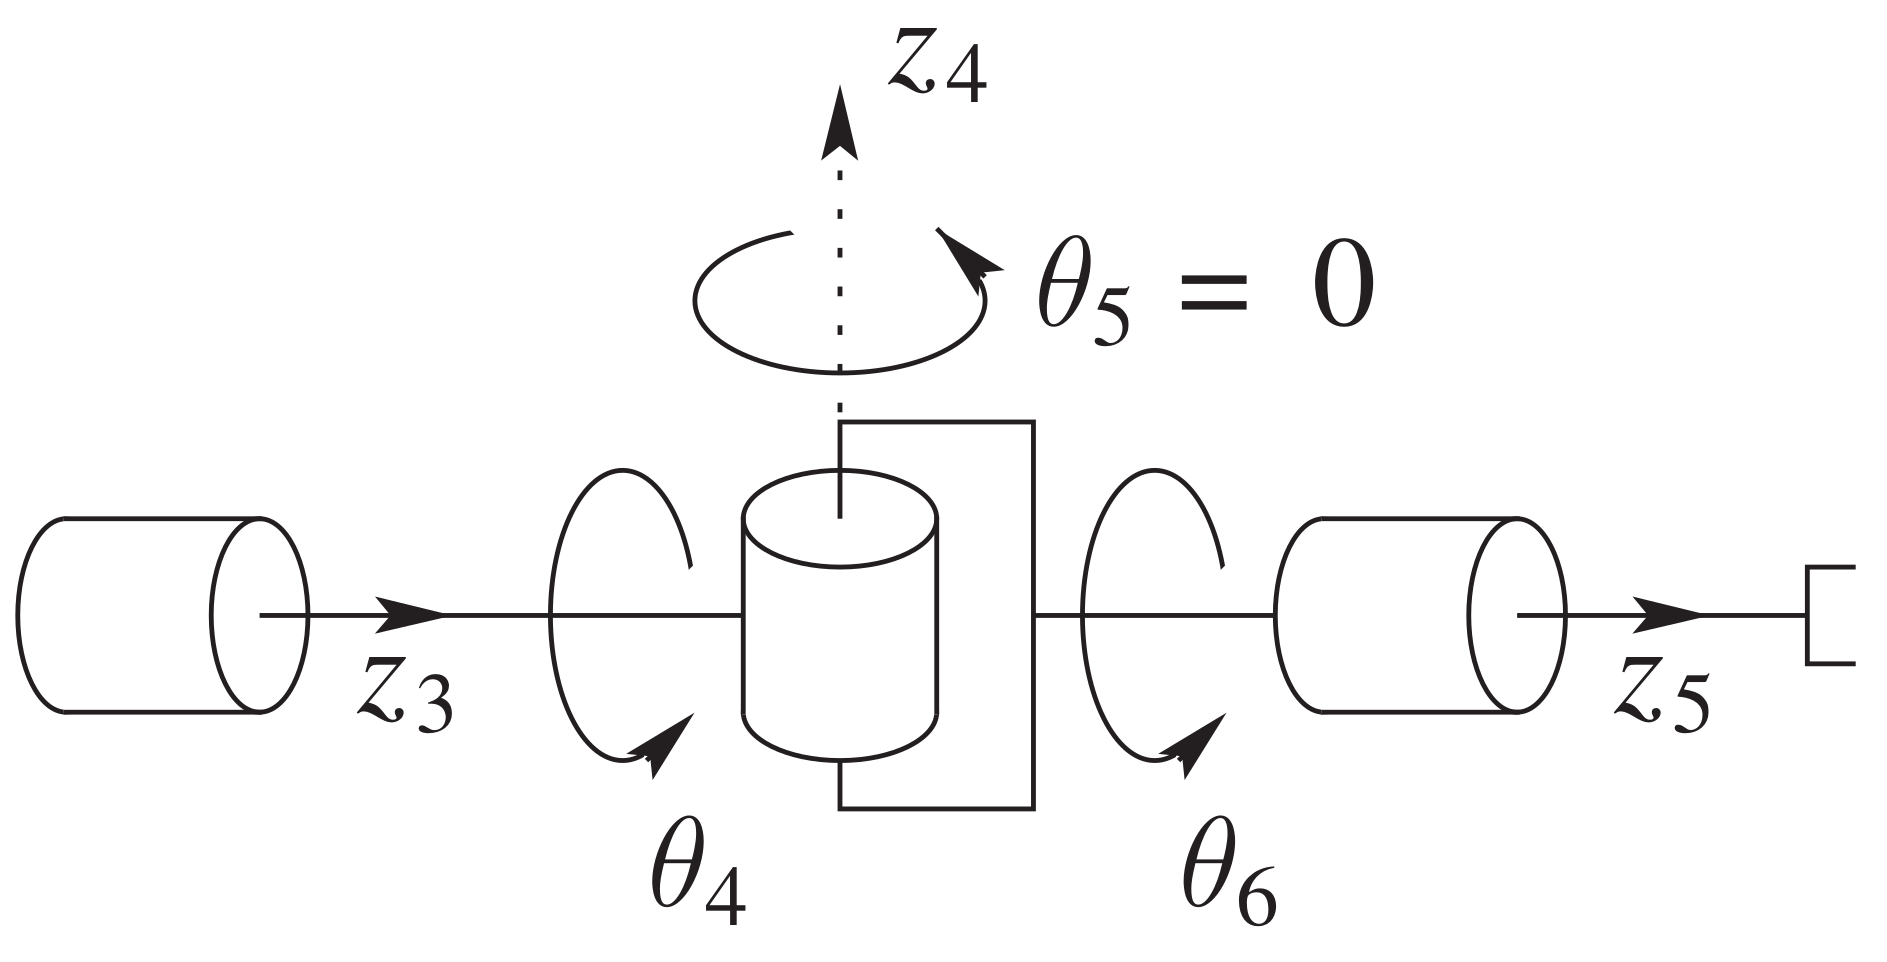
\includegraphics[width=0.85\textwidth]{figures/spherical_wrist_singularity.png} 
                % \caption{\footnotesize }
            \end{figure}
            \vspace{-2mm}
            \centering
            \footnotesize{Spherical wrist singularity}
        \end{column}
    \end{columns}
\end{frame}



\begin{frame}
    \frametitle{Arm Singularities}

    \begin{itemize}
        \item To investigate arm singularities we need only to compute $\det
        J_{11}$, which is done using the equation
        \[ J_{v_i} = 
        \begin{cases}
            z_{i-1} \times (o - o_{i-1}) & \mbox{for revolute joint $i$} \\
            z_{i-1} & \mbox{for prismatic joint $i$}
        \end{cases}    
        \]
        where $o$ is the wrist center.
    \end{itemize}
\end{frame}


\begin{frame}
    \frametitle{Arm Singularities of Elbow Manipulator}

    \begin{itemize}
        \item The three-link articulated manipulator has the determinant $J_{11}$
        \[
            J_{11} = \bmat{
                -a_2s_1c_2 - a_3s_1c_{23} & -a_2s_2c_1 - a_3s_{23}c_1 & -a_3c_1s_{23} \\ 
                a_2c_1c_2 + a_3c_1c_{23} & -a_2s_1s_2 - a_3s_1s_{23} & -a_3s_1s_{23} \\ 
                0 & a_2c_2 + a_3c_{23} & a_3c_{23}
            }
        \]
    \end{itemize}
    \begin{columns}
        \begin{column}{0.6\textwidth}
            \begin{itemize}
                \item The determinant of $J_{11}$ is 
                \[ \det J_{11} = -a_2a_3s_3(a_2c_2 + a_3c_{23}). \]
            \end{itemize}
        \end{column}
        \begin{column}{0.4\textwidth}
            \begin{figure}[bth]
                \centering
                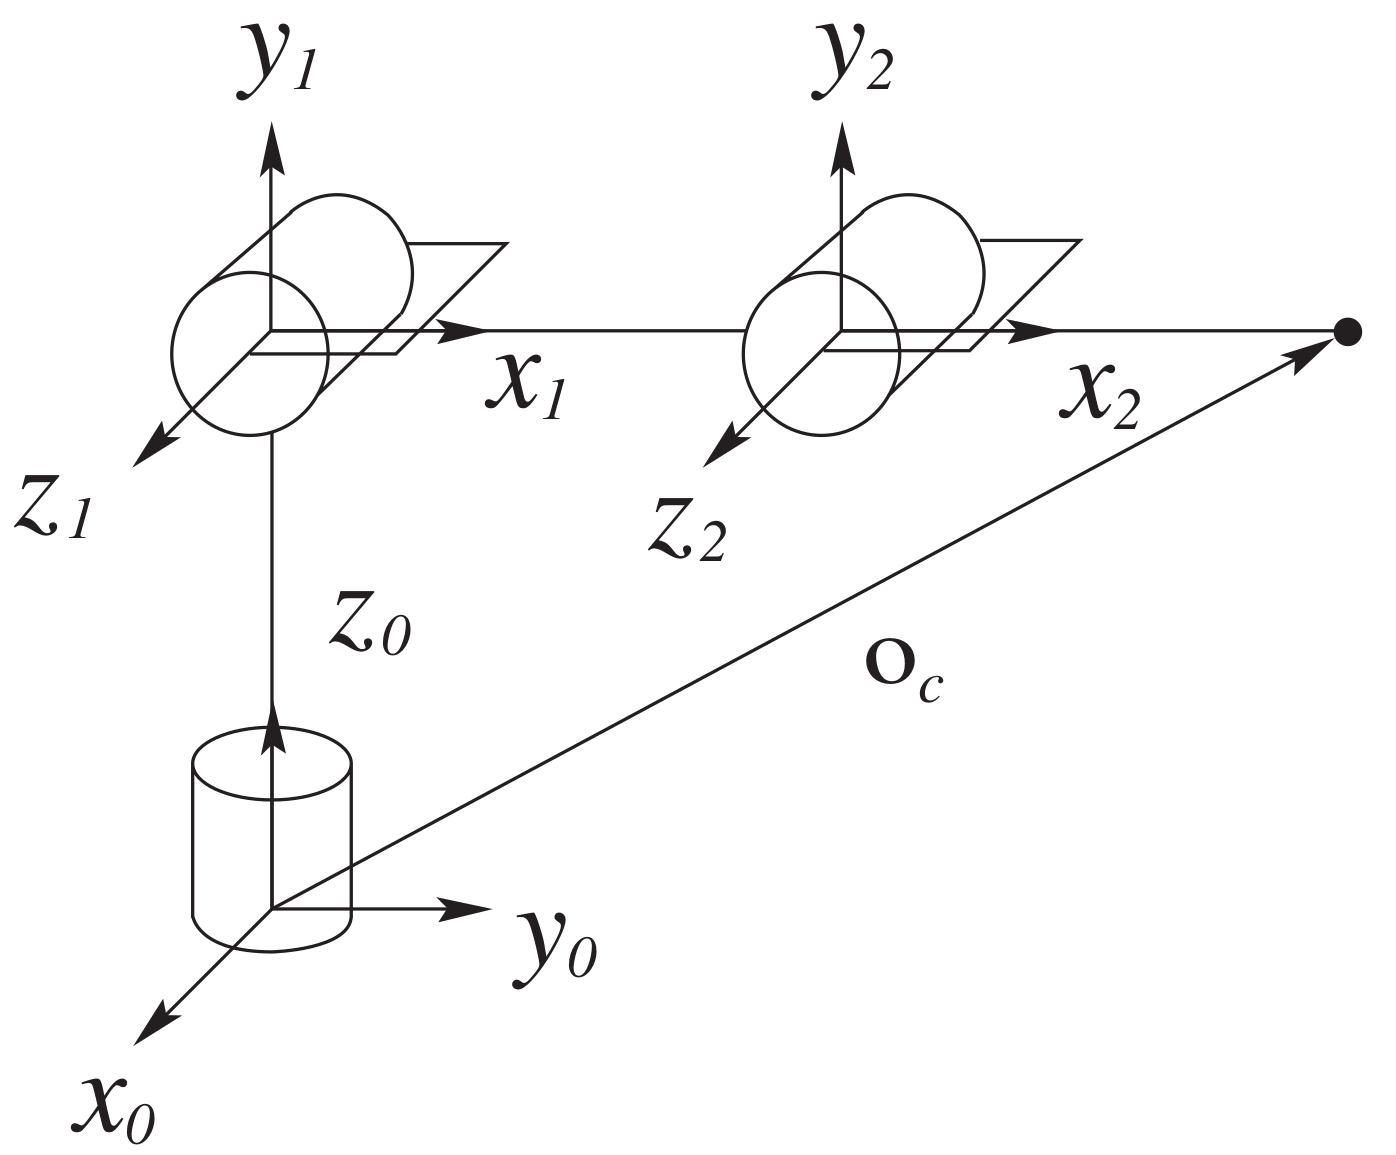
\includegraphics[width=0.85\textwidth]{figures/elbow_manipulator_sing.png} 
                % \caption{\footnotesize }
            \end{figure}
            \vspace{-2mm}
            \centering
            \footnotesize{Elbow manipulator}
        \end{column}
    \end{columns}
\end{frame}


\begin{frame}
    \frametitle{Arm Singularities of Elbow Manipulator}

    \begin{columns}
        \begin{column}{0.6\textwidth}
            \begin{itemize}
                \item We see that the elbow manipulator is
                in a singular configuration when
                \[ s_3 = 0 \Longrightarrow \theta_3 = 0, \pi. \]
                and whenever
                \[ a_2c_2 + a_3c_{23} = 0. \]
                \item The situation of $\theta_3 = 0, \pi$ arises when the elbow
                is fully extended or retracted as shown on the bottom right
                figure.
            \end{itemize}
        \end{column}
        \begin{column}{0.4\textwidth}
            \begin{figure}[bth]
                \centering
                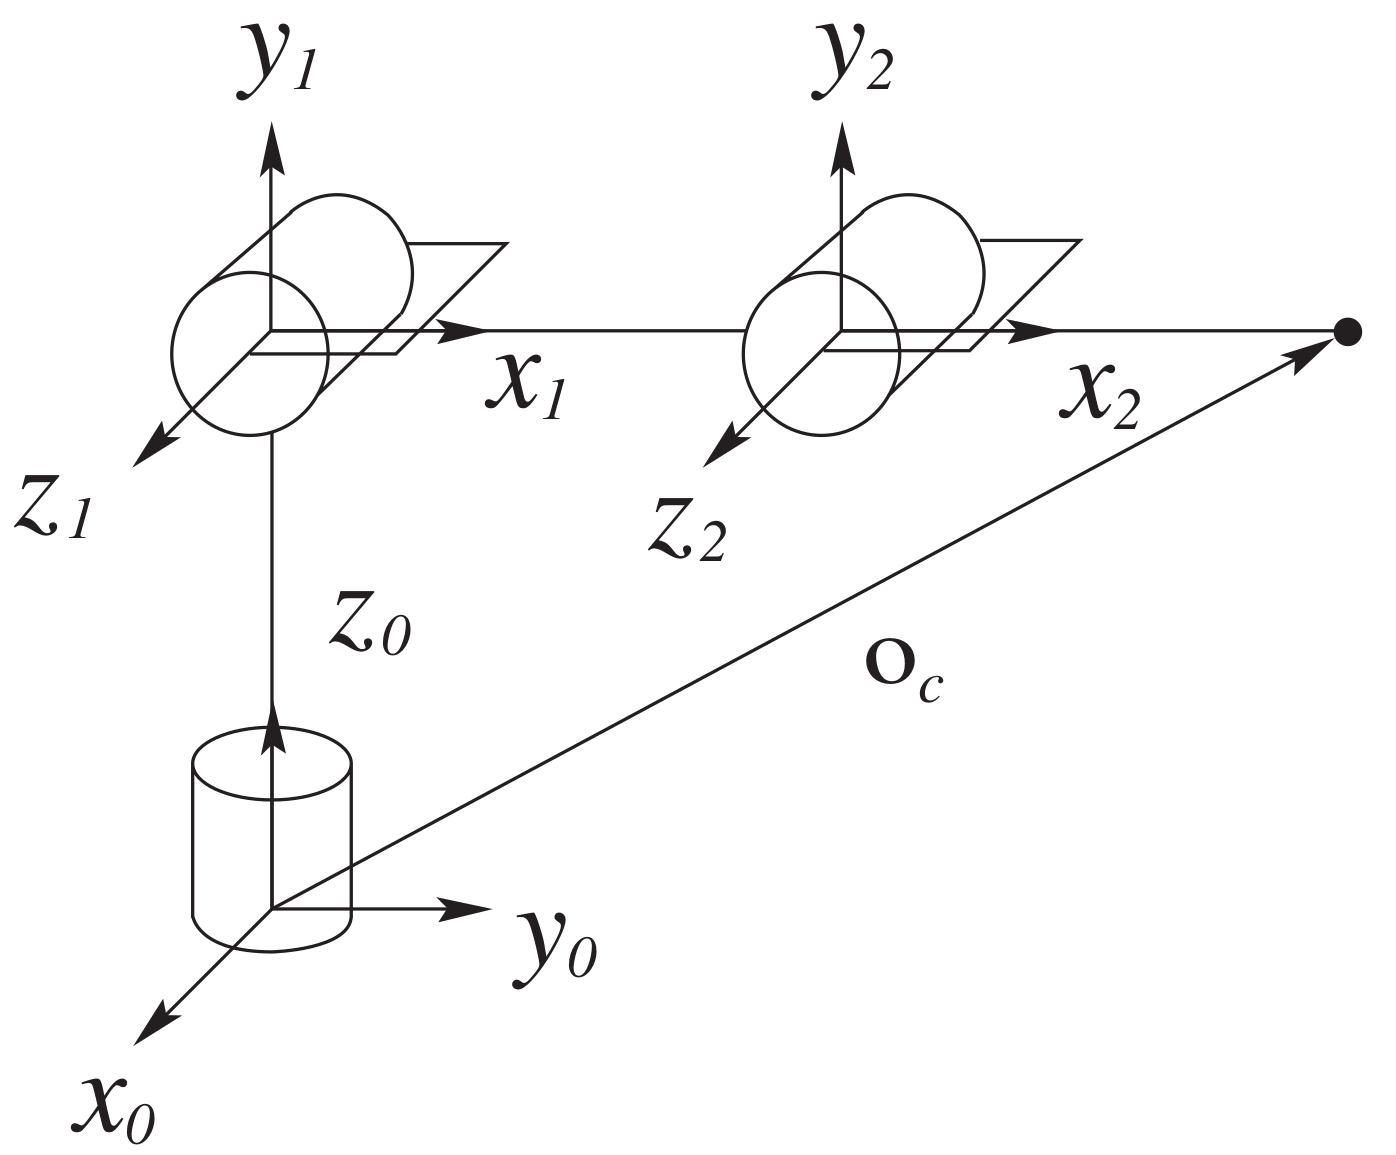
\includegraphics[width=0.85\textwidth]{figures/elbow_manipulator_sing.png} 
                % \caption{\footnotesize }
            \end{figure}
            \vspace{-2mm}
            \centering
            \footnotesize{Elbow manipulator}

            \begin{figure}[bth]
                \centering
                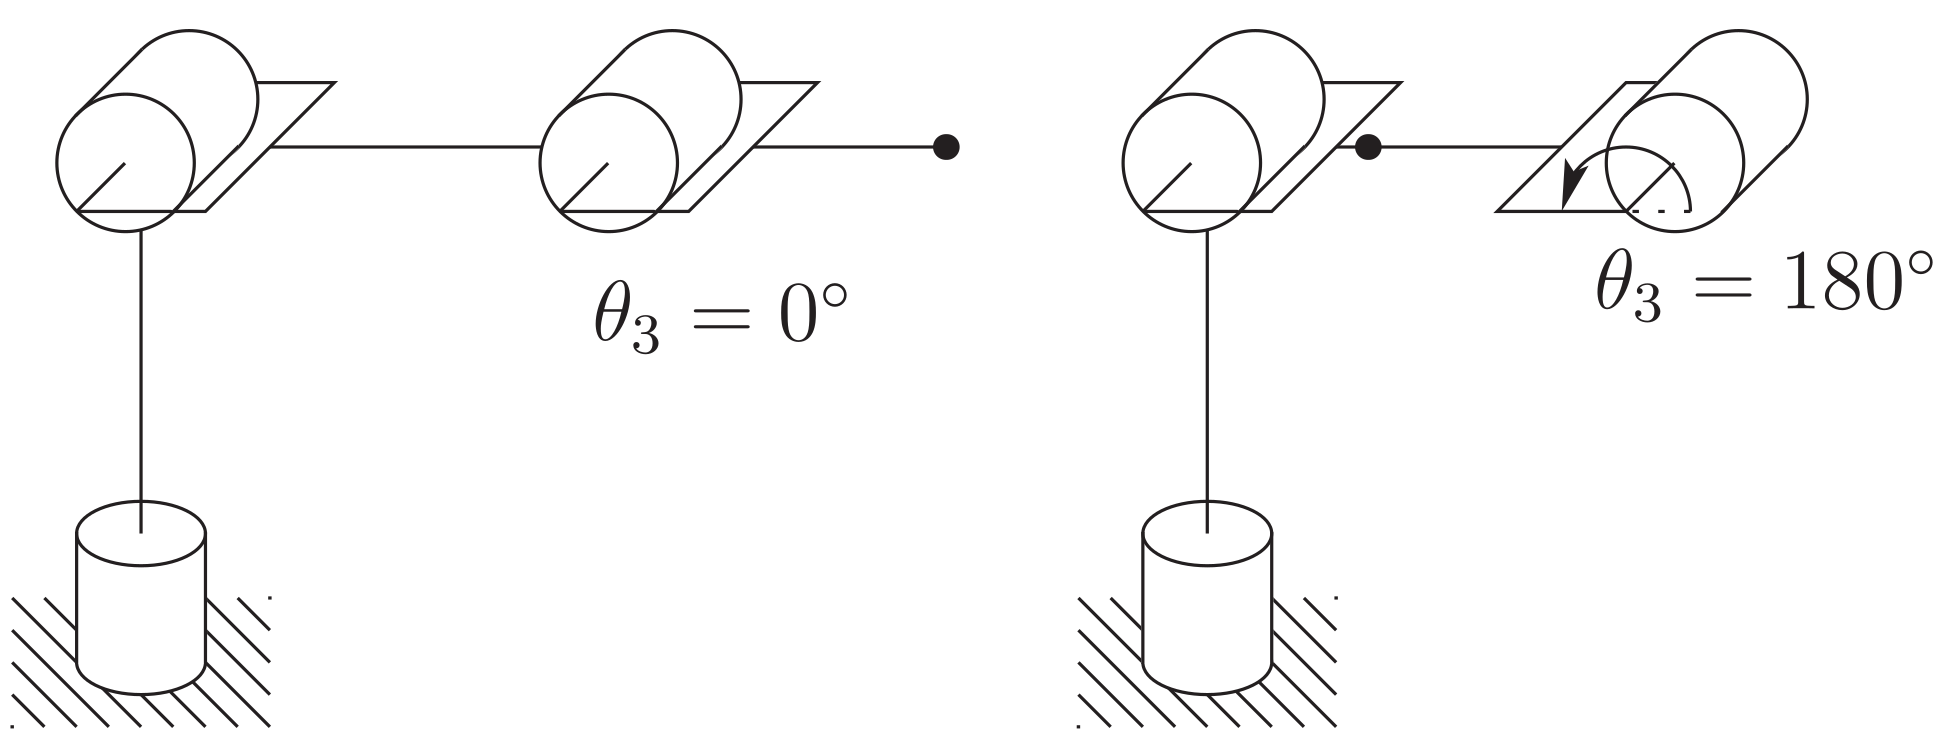
\includegraphics[width=0.85\textwidth]{figures/elbow_singularities.png} 
                % \caption{\footnotesize }
            \end{figure}
            \vspace{-2mm}
            \centering
            \footnotesize{Elbow singularities of the elbow manipulator}
        \end{column}
    \end{columns}
\end{frame}


\begin{frame}
    \frametitle{Arm Singularities of Elbow Manipulator}

    \begin{columns}
        \begin{column}{0.6\textwidth}
            \begin{itemize}
                \item The situation of 
                \[ a_2c_2 + a_3c_{23} = 0. \]
                is shown on the top right figure.
                \item This configuration occurs when the wrist center intersects
                the axis of the base rotation, $z_0$.
                \item If the elbow manipulator has an offset (bottom right
                figure), the wrist center cannot intersect $z_0$.
            \end{itemize}
        \end{column}
        \begin{column}{0.4\textwidth}
            \begin{figure}[bth]
                \centering
                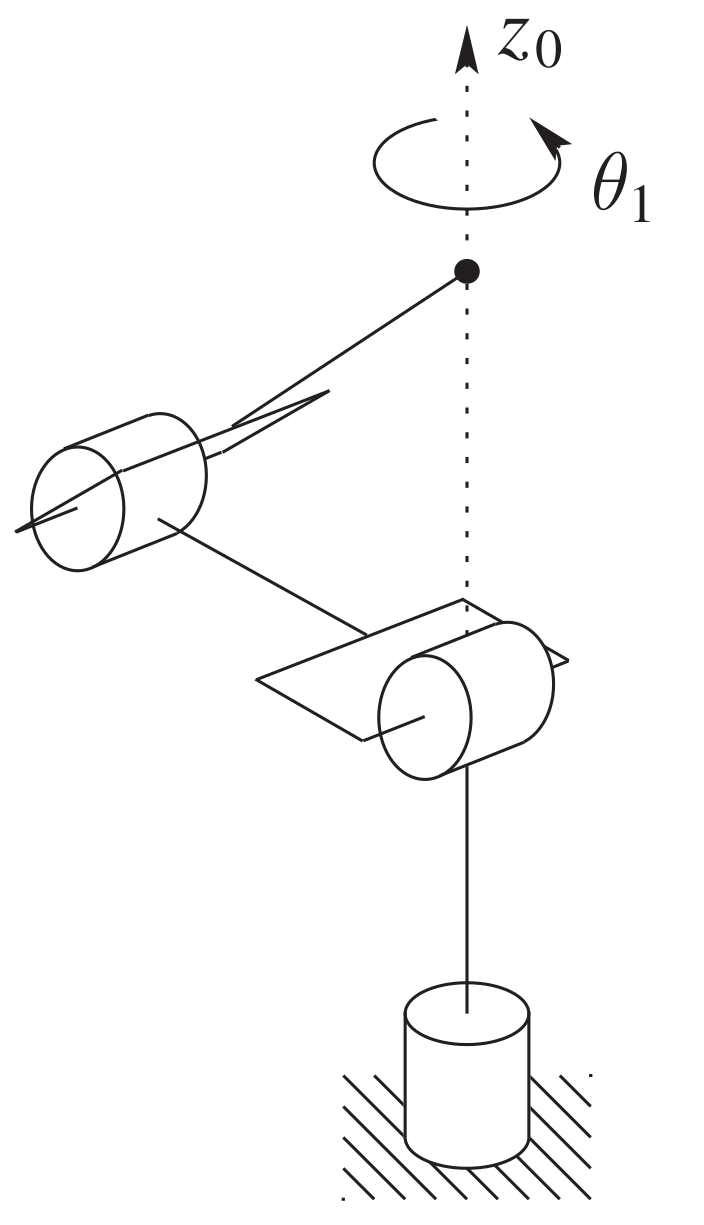
\includegraphics[width=0.4\textwidth]{figures/elbow_sing_no_offset.png} 
                % \caption{\footnotesize }
            \end{figure}
            \vspace{-2mm}
            \centering
            \footnotesize{Singularity of elbow manipulator with no offsets.}

            \begin{figure}[bth]
                \centering
                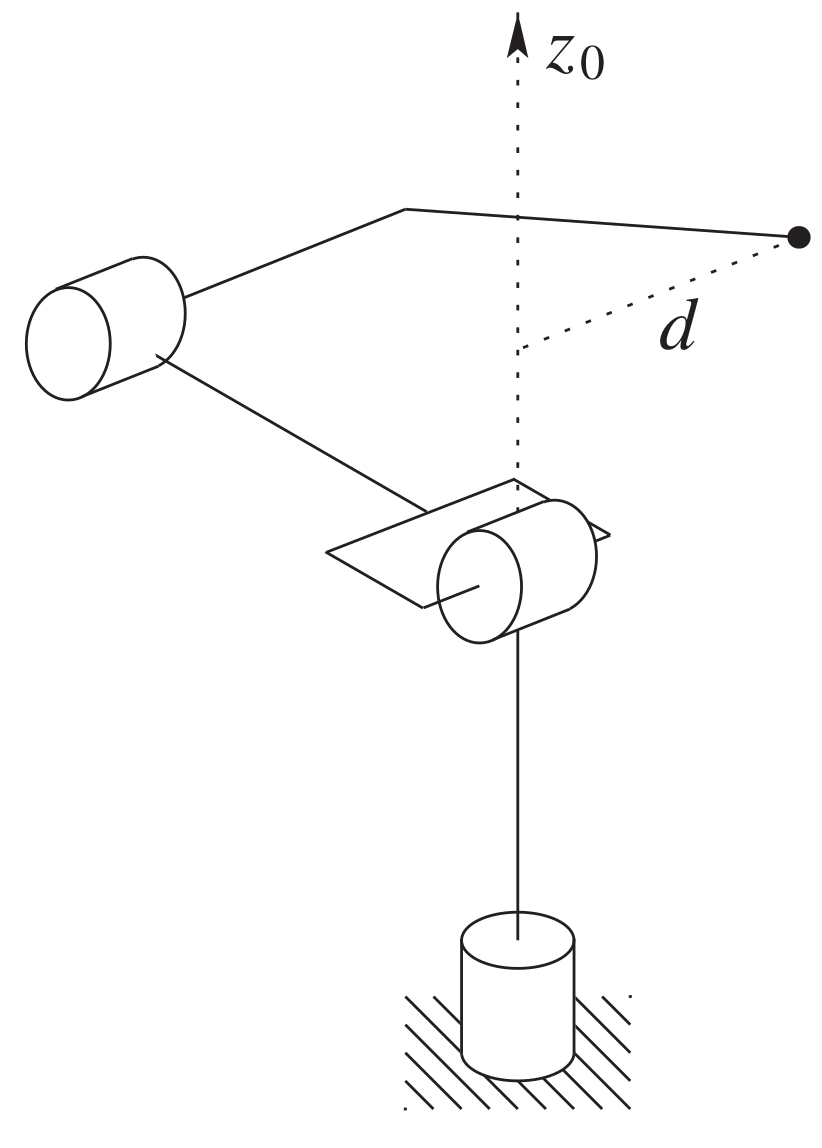
\includegraphics[width=0.4\textwidth]{figures/elbow_sing_w_offset.png} 
                % \caption{\footnotesize }
            \end{figure}
            \vspace{-2mm}
            \centering
            \footnotesize{Elbow manipulator with an offset at the elbow.}
        \end{column}
    \end{columns}
\end{frame}


\endgroup